\chapter{Entwicklung des Prototyps}
\label{ch:development}

Die Umsetzung des Prototyps erfolgt in mehreren Schritten. Zu Beginn wird wie in \ref{sub:unifiedList} beschrieben, die Liste aller Ergebnisse zusammengeführt und absteigend nach der Relevanz sortiert. Anschließend wird der Schlagwortabgleich (\ref{sub:keyword}) implementiert, indem konfigurierbar die Liste der möglichen Synonyme mit dem Suchterm abgeglichen wird und die Ergebnisse geboostet werden, wenn der Suchterm ein Synonym enthält. Zuletzt werden die resultierenden Inhalte nach einem möglichen Vorschlag wie in \ref{sub:suggestion} beschrieben dem Ergebnis hinzugefügt.

\section{Zusammengeführte Liste}
\label{sec:devUnifiedList}

Für die Entwicklung der zusammengeführten Liste im Crossload Frontend ist wichtig, dass die schon implementierte Funktionalität der Suche nach Kategorien nach der Entwicklung immer noch möglich sein muss.
Dazu finden sich auf der Suchergebnisseite mehrere Tabs, bei denen auch eine Suche innerhalb von Kategorien möglich ist.
Sie wird angeführt von der gemischten Suchergebnisseite, auf der wir momentan die Aufteilung in verschiedene Kategorien sehen (\ref{fig:crossloadSuche}).

\begin{figure}[h]
  \begin{centering}
    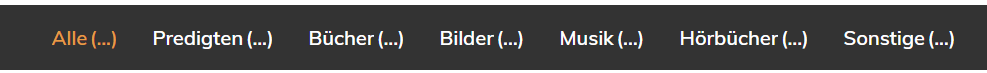
\includegraphics[width=\textwidth]{figures/development/kategorienLeiste.png}
    \caption{Leiste der Suchergebnisse in den verschiedenen Kategorien  \cite{pfleiderer2022}.}
    \label{fig:kategorienLeiste}
  \end{centering}
\end{figure}

Ziel ist es, die gemischte Suchleiste so zu ändern, dass eine große Liste mit allen Kategorien gemischt angezeigt wird.
Dazu wird die bisherige Implementation wie folgt geändert:

Anstatt nach Ergebnissen pro Kategorie abzufragen und diese in den einzelnen Sektionen darzustellen, muss eine gesammelte Anfrage an die Such API gesendet werden.
Diese wird nach dem gegebenen Sortierkriterium, in diesem Fall absteigend nach Relevanzscore sortiert von der Such API zurückgegeben.
Dafür wird zu den vorhandenen Kategorien eine „gemischte“ Kategorie hinzugefügt, bei welcher dann kein Suchfilter mitgegeben wird.
Danach sind nur noch kleine Änderungen notwendig, um das für den Nutzer schön dargestellt zu bekommen.

\begin{lstlisting}[language=Java, title={Erstellen der gemischten Kategorie \cite{crossloadGitlab2022}}]
  export const MIXED_RESULTS_OPTION = {
    category: "mixed",
    path: RESULTS_BASE_URL + "/gemischt",
    lastPathSegment: "gemischt",
    text: "Alle",
    longText: "",
  } as const
\end{lstlisting}

\begin{lstlisting}[language=Java, title={Löschen der Kategorie aus den API Parametern \cite{crossloadGitlab2022}}]
  if (category === "mixed") {
    delete url.category
  }

\end{lstlisting}

% TODO Query anpassen, Erklärung was umgesetzt wurde und grober Screenshot(s) in Anhang


% TODO: Crossload Frontend Suchseite nicht in Kategorien, sondern Komplett.
% TODO: Änderungen zusammenfassen https://gitlab.crossload.org/crossload/frontend/frontend/-/tree/studienarbeit


\section{Schlagwortabgleich}
\label{sec:devKeywords}

% TODO Create configurable Java Parameters mit ausgearbeiteten Schlagwörtern
% TODO For each configuration: Search for Keywords in Search Term
% TODO If found, boost Contents with Category


\section{Vorschläge für weitere Navigation}
\label{sec:devSuggestions}

% TODO Adjust Schema, -> add suggestion object
% TODO Create Function to determine suggestion
% TODO Add Suggestion to result
